\documentclass[spanish]{book}
\usepackage{titlesec}

%Quitar páginas en blanco
\let\cleardoublepage\clearpage
\usepackage{etoolbox}
\makeatletter
\patchcmd{\@endpart}{\vfil\newpage}{\par}{}{}
\makeatother

%\usepackage[spanish]{babel} ¡Esto estaba interfiriendo con las flechitas de los \tikspicture

\renewcommand{\contentsname}{Índice}
\renewcommand{\partname}{Parte}

\titleformat{\chapter}[display]%Ocultar "Chapter"
{\normalfont\huge\bfseries}{}{0pt}{\Huge\thechapter.~}

\titleformat{name=\chapter,numberless}[display]
{\normalfont\huge\bfseries}{}{0pt}{\Huge}
\renewcommand{\chaptermark}[1]{\markboth{{} \thechapter: #1}{}}%Que el número del capítulo salga junto al  del capítulo

\usepackage[bookmarks,bookmarksopen,bookmarksdepth=3]{hyperref}
\usepackage{graphicx}
\usepackage{wrapfig}
\usepackage{float}
\usepackage{subcaption}
\usepackage[left=4cm, right=4cm]{geometry}
\usepackage{enumitem}
\usepackage{palatino}
%\usepackage{parskip}
\usepackage{array}%This is used in a table
\usepackage{amsthm}
\usepackage{amssymb}
%\usepackage{mathabx}
\usepackage[nointegrals]{wasysym}%I was getting some problem "\iint already defined"
\usepackage{amsmath}
\usepackage{tikz}
\usepackage{tikz-cd}
\usetikzlibrary{%
	matrix,%
	calc,%
	arrows,%
	shapes,
	decorations.markings
}

\hypersetup{
	colorlinks=true,
	urlcolor=magenta,
	linkcolor=magenta,
	citecolor=magenta,
	filecolor=blue,
	urlbordercolor=white,
	linkbordercolor=white,
	citebordercolor=white,
	filebordercolor=white
}

\theoremstyle{definition}
\renewcommand{\proofname}{Demostración}
\newenvironment{Proof}[1][Proof]%Proof within proof
{\proof[#1]\leftskip=1cm\rightskip=1cm}{\endproof}

\newtheorem*{defn}{Definición}
\newtheorem{defs}{Definiciones}
\newtheorem*{lema}{Lema}
\newtheorem*{obs}{Observación}
%\newtheorem*{teo}{Teorema}
\newtheorem*{prop}{Proposición}
\newtheorem*{coro}{Corolario}
\newtheorem*{ejer}{Ejercicio}
\newtheorem*{ejem}{Ejemplo}
\newtheorem*{ejems}{Ejemplos}
\newtheorem*{pregunta}{Pregunta}

\usepackage{mdframed}
\newmdtheoremenv{teo}{Teorema}



\newcommand{\R}{\mathbb{R}}
\newcommand{\Z}{\mathbb{Z}}
\newcommand{\N}{\mathbb{N}}
\newcommand{\C}{\mathbb{C}}
\newcommand{\Q}{\mathbb{Q}}
\newcommand{\T}{\mathbb{T}}
\newcommand{\K}{\mathbb{K}}
\DeclareMathOperator{\img}{img}
\DeclareMathOperator{\ran}{ran}
\DeclareMathOperator{\Fix}{Fix}
\DeclareMathOperator{\Stab}{Stab}
\DeclareMathOperator{\MOLS}{MOLS}
\DeclareMathOperator{\STS}{STS}

\DeclareRobustCommand{\stirling}{\genfrac\{\}{0pt}{}}

\title{Notas de Combinatoria}
\author{
\href{https://github.com/danimalabares/combi}{github.com/danimalabares/combi}}

\begin{document}
	\maketitle
	\addcontentsline{toc}{part}{\contentsname}
	\tableofcontents
	
\part{Conteo}
\chapter{Conjuntos y multiconjuntos}\label{chap:set-multiset}
	\begin{prop}
		La cantidad de $k$-subconjuntos de un $n$-conjunto es \[{n\choose k}=\frac{n!}{(n-k)!k!}\]
	\end{prop}
	\begin{defn}
		Escoger $k$ objetos de $n$ tipos sin orden ni límite de repetición produce un \textbf{multiconjunto} de tamaño $k$. Se trata de un conjunto formado por elementos en $[n]$ donde podemos considerar cualquier elemento más de una vez.
	\end{defn}
	\begin{obs}
		Denotemos a cada elección de $k$ números del conjunto $[n]=\{1,\ldots,n\}$ por el vector $(x_1,\ldots,x_n)$ donde $x_i$ es la cantidad de veces que se tomó el $i$-ésimo objeto, es decir, la \textbf{multiplicidad} de cada elemento. Entonces, $\sum_{i=1}^n=k$.
	\end{obs}
	\begin{teo}\label{thm:thm1}
		El número de $k$-multiconjuntos de $[n]$ (equivalentemente, la cantidad de soluciones enteras no negativas de $\sum_{i=1}^nx_i=k$) es ${k+n-1\choose n-1}={k+n-1\choose k}$.
	\end{teo}
\chapter{Relaciones de recurrencia}
\section{Obteniendo recurrencias}
	\begin{defn}
		Una \textbf{relación de recurrencia} para una sucesión $a_0,a_0,\ldots$ es una expresión de la forma $a_n=g(n,a_{n-1},a_{n-2},\ldots,a_0)$, y tiene \textbf{orden} $k$ si sólo depende de los $k$ términos anteriores a $a_n$, es decir, de $a_{n-1},\ldots,a_{n-k}$.
		
		La recurrencia \[a_n=g_{1}(n)a_{n-1}+g_{2}(n)a_{n-2}+\ldots+g_ka_{n-k}+f(n)\]
		es \textbf{lineal} si las funciones $g_i$ y $f$ no dependen de ningún elemento en el espacio lineal generado por la sucesión, $\langle a\rangle$. Si $f$ es cero, es una relación \textbf{homogénea}.
	\end{defn}
	\begin{defn}
		Los \textbf{números de Fibonacci} están dados por la recurrencia
		\[F_{n+2}=F_{n+1}+F_n\qquad F(0)=0,F(1)=1\]
		y los \textbf{números de Fibonacci ajustados} por
		\[\hat{F}_{n+2}=\hat{F}_{n+1}+\hat{F}_n\qquad \hat{F}_0=\hat{F}_1=1\]
		Por último, los \textbf{números de Lucas} son la misma relación de recurrencia pero con
		\[L_1=1,L_2=3\]
		(El término ``números de Fibonacci" fue popularizado por Lucas).
		
	\end{defn}
	\begin{defn}
		Un \textbf{desarreglo} es una permutación sin puntos fijos.
	\end{defn}
\section{Métodos para encontrar soluciones}
\subsection{Relaciones homogéneas}
	\begin{defn}
		Para una relación de recurrencia lineal con coeficientes constantes
		\begin{equation}\label{ec:2.2.1}
			a_n=c_1a_{n-1}+\ldots+c_ka_{n-k}
		\end{equation}
		definimos el \textbf{polinomio característico} como $\phi(x)=x^k-c_1x^{k-1}-\ldots-c_kx^{0}$, y la \textbf{ecuación característica} como $\phi(x)=0$, es decir
		\[x^k=c_1x^{k-1}+\ldots+c_kx^{0}\]
		 cuyas soluciones son las \textbf{raíces características}.
	\end{defn}
	Para entender cómo se usan estos conceptos, primero revisamos el caso sencillo de la recurrencia
	\[a_n=\alpha a_{n-1}\]
	Sustituyendo una y otra vez, obtenemos que $a^n=\alpha a_{n-1}=\alpha^2a_{n-2}=\ldots=\alpha^na_0$. O sea que la solución al final depende de una constante $A$ determinada por la condición inicial y el valor $\alpha$, que es justamente uns raíz de la ecuación característica $x=\alpha$.
	
	En el caso que nos interesa, la ecuación \eqref{ec:2.2.1}, tomemos una raíz característica $\alpha$ y sustituyámosla en la ecuación característica para obtener
	\[\alpha^k=c_1\alpha^{k-1}+\ldots+c_k\alpha^{0}\]
	Y multiplicando por $\alpha^{n-k}$,
	\[\alpha^n=c_1\alpha^{n-1}+\ldots+c_k\alpha^{n-k}\]
	O sea que una solución es $a_n=\alpha^n$. Y como al multiplicar por cualquier constante $A$ se sigue preservando la igualdad, de hecho $a_n=A\alpha^n$ es una solución.
	
	Y si hay otra raíz característica $\beta$ con una solución asociada $a_n=B\beta^n$, de hecho cualquier expresión de la forma $a_n=A\alpha^n+B\beta^n$ también es una solución. (Ver \hyperref[prop:2.2.2.1.1]{la primera proposición} del Deja Vu).
	
	Y para encontrar los valores de $A$ y $B$, es buena idea sustituir en $n=0$.
	
	O sea que la receta es:
	\begin{enumerate}
		\item Busco una constante $\alpha$ tal que $a_n=\alpha^n$ sea una solución. Esto naturalmente me lleva a la ecuación característica.
		\item Las raíces me dan las soluciones de la recurrencia en la siguiente forma:
	\begin{teo}[Solución General]
		Una recurrencia homogénea lineal de orden $k$ con coeficientes constantes cuyas raíces características son $\alpha_1,\ldots,\alpha_r$, todas distintas y con multiplicidades $d_1,\ldots,d_r$, tiene solución
		\[a_n=\sum_iP_i(n)\alpha_i^n\]
		donde cada $P_i$ es un polinomio de grado menor que $d_i$.
	\end{teo}
	(De hecho, todas las soluciones son de esta forma cambiando la elección de los $P_i$.)
	\item Encuentro los valores de los polinomios (muchas veces son constantes, cuando las multiplicidades son 1) sustituyendo en las condiciones iniciales que nos dieron.
\end{enumerate}	

\iffalse
\subsection{Déjà Vu de Ecuaciones diferenciales}
	Referencias: \href{http://www.cds.caltech.edu/~murray/courses/cds101/fa02/precourse/delvecchio-26sep02.pdf}{esto} y \href{https://tutorial.math.lamar.edu/Classes/DE/SolutionsToSystems.aspx#mjx-eqn-eqeq1}{esto}.
	\begin{defn}Un sistema de ecuaciones diferenciales lineales
	\begin{equation}\label{ec:2.2.1.1}
		\dot{\mathbf{x}}=\mathbf{A}\mathbf{x}+\mathbf{f}
	\end{equation}
	se llama \textbf{homogéneo} si el vector $\mathbf{f}=0$.
	\end{defn}

	\begin{defn}El \textbf{polinomio característico} de $\mathbf{A}$ es una función de $\lambda$ dada por $\det(\lambda \mathbf{Id}-\mathbf{A})$. Las raíces de este polinomio son los \textbf{valores propios} de $\mathbf{A}$, y los \textbf{vectores propios} son las soluciones de $(\mathbf{A}-\lambda \mathbf{Id})\mathbf{v}=0$.
	\end{defn}
	\begin{teo}
		Si los valores propios de una matriz $\mathbf{A}$ de $n\times n$ son reales y diferentes, entonces la matriz formada por cualquier conjunto de vectores propios $\mathbf{v}_1,\ldots,\mathbf{v}_n$, digamos $\mathbf{P}=(\mathbf{v}_1,\ldots,\mathbf{v}_n)$ es invertible y
			\[\mathbf{PAP}^{-1}=\mathbf{\Lambda}\]
		es diagonal.
	\end{teo}
	
	Para el problema homogéneo
		\begin{equation}\label{ec:2.2.1.2}
		\dot{\mathbf{x}}=\mathbf{A}\mathbf{x}
	\end{equation}
	consideremos el cambio de coordenadas
	\[\mathbf{z}=\mathbf{P}^{-1}\mathbf{x}\]
	que al derivar nos lleva a que
	\[\dot{\mathbf{z}}=\mathbf{P}^{-1}\dot{\mathbf{x}}=\mathbf{P}^{-1}\mathbf{A}\mathbf{x}=\mathbf{PAP}^{-1}z=\mathbf{\Lambda z}\]
	Así que si $\lambda_1,\ldots,\lambda_n$ son los valores propios, el problema en las nuevas coordenadas se reduce a
	\[z_i=\lambda_i z_i\]
	que tiene solución
	\[z_i=z_i(0)e^{\lambda_it}\]
	
	\begin{prop}\label{prop:2.2.2.1.1}
		Si $\mathbf{x}_1$ y $\mathbf{x}_2$ son soluciones de \eqref{ec:2.2.1.2}, entonces
		\[c_1\mathbf{x}_1+c_2\mathbf{x}_2\]
		también lo es.
	\end{prop}
	\begin{prop}
		Si $\mathbf{x}_1,\ldots,\mathbf{x}_n$ son soluciones de un sistema de ecuaciones diferenciales de $n\times n$ tales que
		\[\det((\mathbf{x}_1,\ldots,\mathbf{x}_n))\neq0\]
		entonces, se trata de un \textbf{conjunto fundamental de soluciones} y de hecho cualquier solución es de la forma
		\[c_1\mathbf{x}_1+\ldots+c_n\mathbf{x}_n\]
	\end{prop}
\newpage

\subsection{Déjà Vu de Ecuaciones diferenciales 2}
Usando \href{https://tutorial.math.lamar.edu/Classes/DE/NonhomogeneousDE.aspx#mjx-eqn-eqeq1}{estas notas} como guía, consideremos la siguiente ecuación diferencial no homogénea:
\begin{equation}\label{2.2.3.1}
	\ddot{y}+p(t)\dot{y}+q(t)y=f(t)
\end{equation}
y la ecuación homogénea asociada:
\begin{equation}\label{2.2.3.2}
	\ddot{y}+p(t)\dot{y}+q(t)y=0
\end{equation}
Resulta que:
\begin{teo}
	Si $Y_1(t), Y_2(t)$ son soluciones de \eqref{2.2.3.1} y $y_1(t),y_2(t)$ son un conjunto fundamental de soluciones de \eqref{2.2.3.2}, entonces
	\[Y_1(t)-Y_2(t)\]
	también es solución de \eqref{2.2.3.2} así que se puede escribir como
	\[Y_1(t)-Y_2(t)=c_1y_1(t)+c_2y_2(t)\]
\end{teo}
	Para aplicar este teorema, necesitamos una solución particular de \eqref{2.2.3.1}, digamos $Y_P(t)$. Supongamos que $y(t)$ es la solución general que buscamos. Luego,
	\[Y_P(t)-y(t)\]
	es una solución del sistema homogéneo asociado, así que se puede escribir como 
	\begin{align*}
		y(t)-Y_P(t)&=c_1y_1(t)+c_2y_2(t)\\
	\iff y(t)&=c_1y_1(t)+c_2y_2(t)+Y_P(t)
	\end{align*}
	para algún conjunto fundamental de soluciones del homogéneo.
\fi
\subsection{Relaciones no homogéneas}
	Literalmente es lo mismo que para ecuaciones diferenciales: las soluciones de una relación de recurrencia no homogénea están dadas por
	\[a_n=p_n+h_n\]
	donde $p_n$ es una solución particular y $h_n$ es una solución del sistema homogéneo asociado.
	
	Para encontrar la solución particular consulté \href{https://courses.ics.hawaii.edu/ReviewICS241/morea/counting/RecurrenceRelations2-QA.pdf}{estas notas hawaiianas}. Resulta que para una recurrencia de la forma
	\[a_n=c_1a_{n-1}+\ldots+c_k+F(n)\]
	donde $F(n)=(b_dn^d+\ldots+b_1n+b_0)s^n$ para ciertos números reales $b_d,\ldots,b_0,s$, hay de dos sopas:
	\begin{enumerate}
		\item Cuando $s$ no es una raíz del polinomio característico de la homogénea. En este caso hay una solución particular de la forma
		\[(\alpha_dn^d+\ldots+\alpha_1n+\alpha_0)s^n\]
		
		\item Cuando $s$ es una raíz de multiplicidad $m$ del polinomio característico de la homogénea. En este caso hay una solución particular de la forma
		\[n^m(\alpha_dn^d+\ldots+\alpha_1n+\alpha_0)s^n\]
		
	\end{enumerate}
	
	Siguiendo a West:
	\begin{teo}
		Tomemos una recurrencia de la forma $a_n=(\sum_{i=1}^kc_ia_{n-i})+F(n)\alpha^n$ donde $n\geq k$, $F$ es un polinomio de grado $d$, y $\alpha$ es una raíz de multiplicidad $r$ de la recurrencia homogénea asociada.
		
		Entonces existe una solución de la forma $a_n=P(n)n^r\alpha^n$ donde $P$ es un polinomio de grado a lo más $d$.
	\end{teo}

\subsection{Usando funciones generatrices}\label{sec:res-rec-fg}
\begin{defn}
	Dada una sucesión $(a_n)$, una \textbf{función generatriz} es la serie formal $\sum_{n\geq0}a_nx^n$. Y el operador $[x^n]$ nos devuelve el coeficiente que acompaña a $x^n$ en la serie.
\end{defn}
El método para solucionar recurrencias es como sigue:
\begin{enumerate}
	\item Multiplicar simbólicamente por potencias de $x^n$ y sumar todos los términos de la recurrencia en el dominio en el que sea válida.
	
	Por ejemplo, si tenemos $a_n=a_{n-1}+n$ para $n\geq1$ y $a_0=1$, multiplicamos por potencias de $x^n$ y sumamos para obtener
	\[\sum_{n\geq1}a_nx^n=\sum_{n\geq 1}a_{n-1}x^n+\sum_{n\geq1}nx^n\]
	Si $A(x)=\sum_{n\geq0}a_nx^n$, el lado izquierdo es $A(x)-1$. El primer sumando del lado derecho es $xA(x)$.
	
	El segundo sumando se simplifica así: como
	 \[1+x+x^2+x^3+\ldots=\sum_{n\geq0}x^n=\frac{1}{1-x}\]
	al derivar esta expresión obtenemos que
	\[1+2x+3x^2+\ldots=\frac{d}{dx}\frac{1}{1-x}=-\frac{1}{(1-x)^2}\]
	así que el segundo término de la suma es $-\frac{x}{(1-x)^2}$. Tenemos que
	\begin{align*}
		A(x)-1&=xA(x)-\frac{x}{(1-x)^2}\\ A(x)-xA(x)&=1-\frac{x}{(1-x)^2}\\
		A(x)(1-x)&=1-\frac{x}{(1-x)^2}\\
		A(x)&=\frac{1}{1-x}-\frac{x}{(1-x)^3}\\
		A(x)&=\sum_{n\geq0}x^n-\sum_{n\geq0}{n+2\choose 2}x^n\\
		&=\sum_{n\geq1}x^n-\sum_{n\geq1}{n+2\choose 2}x^n\\
	\end{align*}
	Suponiendo que conocemos la expansión de $\frac{x}{(1-x)^3}$. En fin, $a_n=1-{n+2\choose 2}$.
	\begin{ejer}
		Resolver la recursión de Fibonacci con este método. (Ver \textbf{generatingfunctionology}, p. 9)
	\end{ejer}
	
\end{enumerate}
\chapter{Funciones generatrices}
\section{Ordinarias}
\begin{defn}
	Dada una sucesión $(a_n)$, una \textbf{función generatriz ordinaria} es la serie formal $\sum_{n\geq0}a_nx^n$. Y el operador $[x^n]$ nos devuelve el coeficiente que acompaña a $x^n$ en la serie. Si el número $a_n$ representa la cantidad de cosas $u$ en cierto universo $U$ que tienen peso $w(u)$ igual a $n$, decimos que la función generatriz es el \textbf{enumerador dado por $w$ para $U$}.
\end{defn}
\begin{ejem}
	La función generatriz de la sucesión $a_n=n$ es $\sum_{n=0}^\infty nx^n$, que, como vimos en la sección de \hyperref[sec:res-rec-fg]{solución de recurrencias}, se puede ver como $x\frac{d}{dx}\frac{1}{1-x}=\frac{x}{(1-x)^2}$. Esta clase de expresiones nos permiten manipular y extraer información de las sucesiones.
\end{ejem}
\begin{defn}
	La \textbf{suma} y el \textbf{producto} de las funciones generatrices ordinarias $\sum_{n=0}^\infty a_nx^n$ y $\sum_{n=0}^\infty b_nx^n$ están dados por 
	\[\sum_{n=0}^\infty (a_n+b_n)x^n\qquad\text{y}\qquad\sum_{n=0}^\infty \left(\sum_{i+j=n}a_ib_j\right)x^n=\sum_{n=0}^\infty \left(\sum_{j=0}^na_jb_{n-j}\right)x^n\]
\end{defn}
\begin{lema}
	Si las funciones generatrices de $(a_n)$ y $(b_n)$ cuentan los objetos que tienen peso $n$ en los universos $A$ y $B$ (son enumeradores),
	entonces su producto es el enumerador de las parejas de objetos en $A\times B$ tales que sus pesos suman $n$.
\end{lema}
\begin{coro}
	Haciendo inducción sobre el lema anterior, vemos que si $(a^1_n),\ldots,(a^r_n)$ son sucesiones que representan cuántos objetos con peso $n$ hay en los conjuntos $A_1,\ldots,A_r$, entonces, el $k$-ésimo coeficiente de la función generatriz del producto cuenta las $r$-tuplas tales que la suma de los pesos es $k$.
\end{coro}
\begin{ejem}
	Recordemos que un $k$-multiconjunto construido a partir de $n$ elementos está determinado por una $n$-tupla donde cada entrada es la multiplicidad de cada elemento, y estas multiplicidades deben sumar $k$. 
	
	Para encontrar un enumerador de los $k$-multiconjuntos formados con $n$ números, podemos considerar el producto de $n$ enumeradores que cuentan los $k$-multiconjuntos construidos a partir de cada uno de los $n$ elementos.
	
	Pero claro, sólo hay un $k$-multiconjunto que se puede formar a partir de un elemento: el que está formado por $k$ copias del elemento. Así, el enumerador de los multiconjuntos formados a partir de un sólo elemento es $\sum_{k=0}^\infty x^k$.
	
	Luego, el enumerador de los $k$-multiconjuntos es $\left(\sum_{k=0}^\infty x^k\right)^n$. Y recordando el teorema que mostramos en el \hyperref[chap:set-multiset]{capítulo 1}, concluimos que
	\[(1+x+x^2+\ldots)^n=\sum_{k=0}^\infty {k+n-1\choose n}x^k\]
	Llevemos un poco más lejos este razonamiento: el producto de $1-x$ y $\sum_{k=0}^\infty x^k$ es 1, así que $(1-x)^n\left(\sum_{k=0}^\infty x^k\right)^n=1^n=1$. Luego,
	\[\frac{1}{(1-x)^n}=\sum_{k=0}^\infty {k+n-1\choose n}x^k\]
	\textcolor{cyan}{... ¿qué no era más fácil sólo decir $(1+x+x^2+\ldots)=\frac{1}{1-x}$?}
\end{ejem}
\begin{ejem}[Multiplicidades restringidas]\label{restr}
	A veces queremos restringir alguno de los elementos a que aparezca cierta cantidad de veces. En estos casos, el enumerador individual de este elemento debe ser $\sum_{k\in S}x^k$.
	
	Por ejemplo, si todos los elementos se deben usar al menos una vez, tenemos:
	\[(x+x^2+x^3+\ldots)^n=\left(\frac{x}{1-x}\right)^n\]
	Y luego:
	\[[x^k]\left(\frac{x}{1-x}\right)^n=[x^{k-n}]\frac{1}{(1-x)^n}={k-n+n-1\choose n-1}={k-1\choose n-1}\]
\end{ejem}
Agregemos aquí:
\begin{teo}[Regla 5]\label{rule5}
	Si $f\overset{ops}{\longleftrightarrow}\{a_n\}_0^\infty$  \[\frac{f}{1-x}\overset{ops}{\longleftrightarrow}\left\{\sum_{j=0}^na_j\right\}_{n\geq0}\]
\end{teo}
\section{F.g. exponenciales}
\begin{defn}
	La \textbf{función generatriz exponencial (fge)} de una sucesión $(a_n)$ es $\sum a_{n}x^{n}/n!$.
\end{defn}
\begin{ejem}
	La cantidad de palabras de longitud $n$ formadas con un alfabeto de $k$ letras es $k^n$. La función generatriz exponencial correspondiente tiene la expresión muy sencilla $e^{kx}$.
\end{ejem}
\begin{teo}\label{rule3p}
	Siguiendo la notación del libro \textbf{generatingfunctionology}, si tenemos dos funciones generatrices exponenciales $f\overset{egf}{\longleftrightarrow}\{a_n\}_0^\infty$ y $g\overset{egf}{\longleftrightarrow}\{b_n\}_0^\infty$, entonces su producto está dado por
	\[fg\overset{egf}{\longleftrightarrow}\left\{\sum_k{n\choose k}a_kb_{n-k}\right\}_0^\infty\]
\end{teo}
	En comparación con las funciones generatrices ordinarias, en cuyo caso tenemos que:
		\[fg\overset{ogf}{\longleftrightarrow}\left\{\sum_ka_kb_{n-k}\right\}_0^\infty\]
		
De hecho podemos generalizar este resulado:
\begin{teo}	
	Para $f\overset{egf}{\longleftrightarrow}\{a_n\}_0^\infty$, $g\overset{egf}{\longleftrightarrow}\{b_n\}_0^\infty$ y $h\overset{egf}{\longleftrightarrow}\{c_n\}_0^\infty$
	\[fgh\overset{egf}{\longleftrightarrow}\left\{\sum_{r+s+t=n}\frac{n!}{r!s!t!}a_rb_sc_t\right\}_0^\infty\]
\end{teo}
\begin{teo}	
	Para $f\overset{egf}{\longleftrightarrow}\{a_n\}_0^\infty$,
	\[f^k\overset{egf}{\longleftrightarrow}\left\{\sum_{r_1+r_2+\ldots+r_k=n}\frac{n!}{r_1!r_2!\ldots r_k!}a_{r_1}a_{r_2}\ldots a_{r_k}\right\}_0^\infty\]
\end{teo}
\begin{defn}
	El \textbf{número de Stirling del segundo tipo} $S(n,k)$, también denotado $\stirling{n}{k}$, es la cantidad de particiones de $[n]$ en $k$ bloques no vacíos.
\end{defn}
\begin{teo}
	\[S(n,k)=\frac{1}{k!}\sum_{i=0}^k(-1)^i{k\choose i}(k-i)^n\]
\end{teo}
\begin{proof}
	Primero notemos que las particiones de $[n]$ en $k$ bloques no vacíos se pueden ordenar de acuerdo a los elementos que tienen. Así, podemos ordenar los bloques en la lista $[k]$, y entonces las particiones \textit{ordenadas} $[n]$ en $k$ bloques no vacíos se pueden	ver como funciones suprayectivas de $[n]$ en $[k]$.
	
	También podemos pensar que son palabras de tamaño $n$ en el alfabeto $[k]$, con la \hyperref[restr]{restricción} de que cada letra debe aparecer al menos una vez. Así, la función generatriz exponencial que cuenta la multiplicidad de cada bloque es $\frac{x^1}{1!}+\frac{x^2}{2!}+\frac{x^3}{3!}+\ldots=e^x-1$, y en total, $(e^x-1)^k$ para los $k$ bloques.
	
	Entonces la función generatriz exponencial que cuenta las particiones ordenadas de $n$ elementos en $k$ bloques es $(e^x-1)^k$. Hay $k!$ maneras de ordenar cada $k$ particiones, así que tenemos la ecuación 
	
	\[\sum_{n=0}^\infty k!\stirling{n}{k}\frac{x^n}{n!}=(e^x-1)^k\]
	
	De donde

\end{proof}
\begin{defn}
	El \textbf{número de Bell} $B(n)$ cuenta la cantidad de particiones de $[n]$.
\end{defn}
\begin{ejem}[¿Cuántos desarreglos hay?]
	Recordemos que un \textbf{desarreglo} es una permutación sin puntos fijos. Denotemos por $D_n$ a la cantidad de desarreglos de $n$ elementos.
	
	La cantidad de permutaciones de $n$ elementos, que es $n!$, se puede ver como la suma de las cantidades de permutaciones que no fijan elementos, las que fijan 1 elemento, 2 elementos, etc., hasta la identidad. Cada una de estas cantidades es justamente $D_{n-k}$.
	
	En cada caso hay ${n\choose k}$ elecciones de subconjuntos de $k$ elementos que pueden quedar fijos, así que
	\[n!=\sum_{k=0}^n{n\choose k}D_{n-1}\]
	Diviendo entre $n!$, multiplicando por $x^n$ y sumando sobre todos los naturales, obtenemos las funciones generatrices exponenciales:
	\[\frac{1}{1-x}=e^xD(x)\]
	Usando \hyperref[rule3p]{la regla del producto exponencial}, donde $D(x)$ es la función generatriz exponencial, es decir, $D(x)=\sum_{n\geq0}\frac{D_n}{n!}x^n$.
	
	Usando \hyperref[rule5]{la regla 5} en la expresión $e^{-x}/(1-x)$ obtenemos que $D\overset{egf}{\longleftrightarrow}\left\{\sum_k(-1)^k/k!\right\}$, es decir,
	\[\frac{D_n}{n!}=\sum_{k=0}^n\frac{(-1)^k}{k!}\]
	Y para acordarse:
	\[D_n\approx \frac{n!}{e}\]
\end{ejem}
\begin{defn}
	Los \textbf{números de Catalan} $C_n$ cuentan la cantidad de expresiones de $n$ parejas de paréntesis bien balanceadas.
\end{defn}
Por ejemplo, $C_3=5$ ya que sólo hay:
\[((()))\qquad(()())\qquad()()()\qquad()(())\qquad(())()\]
Los números de Catalan también cuentan:
\begin{itemize}
	\item Los caminos en una cuadrícula de $n\times n$ partiendo de la esquina inferior izquierda a la esquina superior derecha sin pasar por arriba de la diagonal.
	\item Triangulaciones de un $n+2$-ágono usando líneas que no se cruzan.
\end{itemize}

\chapter{Principio de inclusión-exclusión}
La siguiente fórmula es sumamente familiar:
\[|A\cup B|=|A|+|B|-|A\cap B|\]
Y también la generalización para tres conjuntos:
\[|A\cup B\cup C|=|A|+|B|+|C|-|A\cap B|-|A\cap C|-|B\cap C|+|A\cap B\cap C|\]
Que captura la esencia del Principio de Inclusión Exclusión (PIE): \textit{overcounting}, o ``contar de más".

La fórmula general es de alguna manera obvia: la cardinalidad de la unión es igual a la suma de la cardinalidad de cada conjunto, menos las cardinalidades de las intersecciones de a dos, más las intersecciones de a tres, menos las de a cuatro, ..., hasta que sumamos o restamos la intersección de todos (esto depende de la paridad).

Escribir esto puede no ser algo laborioso. Matousek nos da una buena solución de acuerdo a la notación de que ${X\choose k}$ denota la colección de \textit{subconjuntos} de $X$ de tamaño $k$:
\begin{teo}
	Para cualquierquiera conjuntos finitos $A_1,\ldots,A_n$,
	\[\left|\bigcup_{i=0}^nA_i\right|=\sum_{i=1}^n(-1)^{i+1}\sum_{\mathcal{A}\in{\{A_1,\ldots,A_n\}\choose i}}\left|\bigcap \mathcal{A}\right|\]
\end{teo}
Y hay otra expresión ``almost devilish":
\[\left|\bigcup_i^nA_i\right|=\sum_{\emptyset\neq\mathcal{A}\subseteq \{A_1,\ldots,A_n\}}(-1)^{|\mathcal{A}|-1}\left|\bigcap\mathcal{A}\right|\]
Que de hecho es exactamente lo que West denota por $f(\emptyset)$.
\chapter{Enumeración bajo acciones de grupo}
\begin{teo}[Lema que no es de Burnside]
	Dada una acción de un grupo finito $G$ en un conjunto $X$,
	\[|X/G|=\frac{1}{|G|}\sum_{g\in G}|\Fix g|\]
	donde $X/G$ es el conjunto de órbitas y $\Fix g$ es el conjunto de puntos fijos de $g\in G$.
\end{teo}
\begin{proof}
	Primero notemos que 
	\[\sum_{g\in G}|\Fix g|=\sum_{x\in X}|\Stab x|\]
	ya que ambos lados cuentan la cantidad de parejas $(g,x)$ tales que $g$ fija a $x$.
	
	Ahora notemos que, dado $x$, hay tantos elementos en su órbita como clases laterales  $G/\Stab x$. En efecto: la correspondencia $gx\mapsto g+\Stab x$ está bien definida y es biyectiva. Agregando a esto el teorema de Lagrange,
	\[|G\cdot x|=[G:\Stab x]=|G|/|\Stab x|\]
	Invirtiendo este cociente y sumando sobre $x\in X$, casi terminamos. Sólo falta notar que como las órbitas son una partición de $X$,
	\[\sum_{x\in X}\frac{1}{|G\cdot x|}=\sum_{G\cdot x\in G/X}\left(\sum_{y\in G\cdot x}\frac{1}{|G\cdot y|}\right)=\sum_{G\cdot x\in G/X}1=|X/G|\]
\end{proof}
\begin{teo}[de enumeración de Pólya-Redfield]
	Sea $X$ un conjunto finito, $G$ un grupo de permutaciones de $X$ y $Y$ un conjunto finito de colores. Entonces,
	\[|Y^X/G|=\frac{1}{|G|}\sum_{g\in G}|Y|^{c(g)}\]
	donde:
	\begin{itemize}
		\item $Y^X$ es el conjunto de coloraciones de $X$, formalmente el conjunto de funciones $X\to Y$.
		\item Como $G$ actúa en $X$, también actúa en $Y^X$, así que hay un espacio de órbitas $Y^X/G$.
		\item $c(g)$ es la cantidad de ciclos que tiene $g$ cuando lo vemos como una permutación de $X$.
	\end{itemize}
\end{teo}
\begin{obs}
	Hay una versión con pesos de este teorema, que demuestra West. Po ahora no lo escribimos.
\end{obs}
\begin{defn}
	El índice de ciclos es un polinomio
	\[Z_G(x_1,x_2,\ldots)=\frac{1}{|G|}(\text{la función que enlista los elementos en }G\text{ de acuerdo a sus ciclos}\]
	es decir, cada $x_i$ representa un ciclo de longitud $i$.
\end{defn}
Por ejemplo, el polinomio
\[\frac{1}{12}(x^4_1+8x_1x_3+3x^2_2)\]
Es el índice de ciclos del subgrupo de rotaciones de las simetrías de un tetraedro regular, ya que la identidad tiene cuatro 1-ciclos, las rotaciones por el centro de las caras tienen un 1-ciclo y un 3-ciclo, y las rotaciones por los puntos medios de las aristas tienen dos 2-ciclos. Los coeficientes enteros simplemente nos dicen cuántas hay de cada una.

\chapter{Ejercicios}
Los ejercicios vienen de dos libros: W=West, C=Cameron.
\paragraph{W  1.1.1}\textbf{Después de tirar $k$ dados, ¿cuál es la probabilidad de que la suma sea par?}
\begin{proof}[Solución]
	La probabilidad es $1/2$. Denotemos por $P_i$ la probabilidad de que la suma sea par cuando tiramos $i$ dados, y $I_i$ cuando la suma es impar. Entonces, la probabilidad que buscamos, $P_k$, se obtiene de dos formas: cuando al tirar $k-1$ la suma fue par y el $k$-ésimo también salió par, o bien cuando al tirar $k-1$ la suma salió impar y el $k$-ésimo también salió impar. Es decir,
	\[P_k=P_{k-1}\frac{1}{2}+I_{k-1}\frac{1}{2}\]
	Para encontrar $P_{k-1}$, y todos los anteriores, sucederá exactamente lo mismo: \[P_i=P_{i-1}\frac{1}{2}+I_{i-1}\frac{1}{2}\]
	Y de hecho algo análogo pasa con la probabilidad de que la suma sea impar: tiene que ser cierto que los $i-1$ dados anteriores suman par y el $i$-ésimo impar, o bien que los $i-1$ anteriores sumaron impar y el $i$-ésimo par. Es decir, \[I_i=P_{i-1}\frac{1}{2}+I_{i-1}\frac{1}{2}\]
	Hasta que lleguemos a $P_2$, que se obtiene sólo si los dos primeros dados sumaron par, o si los dos sumaron impar, así que $P_2=\frac{1}{2}\frac{1}{2}+\frac{1}{2}\frac{1}{2}=\frac{1}{2}$. Y de hecho $I_2=\frac{1}{2}\frac{1}{2}+\frac{1}{2}\frac{1}{2}=\frac{1}{2}$. Sustituyendo, notemos que $P_3=\frac{1}{2}\frac{1}{2}+\frac{1}{2}\frac{1}{2}=\frac{1}{2}$. Y de hecho esto sigue sucediendo conforme subimos el índice hasta llegar a $k$, es decir, $P_k=\frac{1}{2}\frac{1}{2}+\frac{1}{2}\frac{1}{2}=\frac{1}{2}$
\end{proof}
%\begin{proof}[Solución] 
%	Cada tiro de $k$ dados es una elección de $k$ números, sin límite de repetición y sin importar el orden, del conjunto $[6]=\{1,2,3,4,5,6\}$, es decir, es un $k$-multiconjunto de $[6]$. Por el \hyperref[thm:thm1]{teorema} que vimos, la cantidad de tiros es 
%	\begin{align*}
%		{k+6-1\choose k}&={k+5\choose k}\\
%		&=\frac{(k+5)!}{5!k!}\\
%		&=\frac{(k+5)(k+4)(k+3)(k+2)(k+1)k!}{120\cdot k!}\\
%		&=\frac{(k+5)(k+4)(k+3)(k+2)(k+1)}{120}\\
%		%&=\frac{k^5}{120}+\text{otros términos}+\frac{5!}{120}\\
%		&=\frac{k^5}{120}+\text{otros términos}+1
%	\end{align*}
%	Ahora contemos cuántas de las tiradas son pares. Como impar+impar=par, una tirada puede sumar impar sólo si la cantidad de números impares es impar.
%\end{proof}

\paragraph{W 1.1.2}\textbf{Cuente la cantidad de rectángulos con área positiva formados por una retícula con $m$ rectas horizontales y $n$ verticales}
\begin{proof}[Solución]
	Si contamos sólo los rectángulos actoados, es fácil convencerse de que son $(n-1)(m-1)$. Y los rectángulos no acotados que se forman son $2(m+n)$.
\end{proof}

\paragraph{W 1.1.3}\textbf{El alfabeto romano tiene 21 consonantes y 5 vocales. ¿Cuántas palabras se pueden formar con $r$ consonantes y $s$ vocales?}
\begin{proof}[Solución]
	Una colección de $r$ consonantes entre las 21, sin importar el orden y con posibilidad de repetición es un $r$-multiconjunto de $[21]$, de los que, como sabemos, hay ${r-21-1\choose21-1}={r-20\choose20}$. Análogamente, hay ${s+4\choose4}$ posibles colecciones de vocales que podemos escoger. Ahora sólo queda ordenar los $r+s$ elementos que tenemos.
	
	La respuesta es
	\[{r-20\choose20}{s+4\choose4}(r+s)!\]
\end{proof}

\paragraph{W 1.1.8}\textbf{¿Cuántas manos de 6 cartas se puede formar con una baraja de 52 cartas de forma que haya al menos una carta de cada palo?}
\begin{proof}[Solución]
	$13\cdot13\cdot13\cdot13\cdot48\cdot47$
\end{proof}

\paragraph{W 1.1.9}\textbf{Cuente la cantidad de números enteros del 0 al 99,999 en los que cada dígito se repite a lo más dos veces.}
\begin{proof}[Solución]
	La cantidad de números del 0 al 99,999 es 100,000. Para resolver nuestro problema, basta descartar los números en los que hay al menos un dígito que se repite tres veces. Veamos:
	
	\begin{itemize}
		\item 	La cantidad de números de 5 dígitos tales que todos son diferentes es $10\cdot9\cdot8\cdot7\cdot6$.
		\item Si dos números son iguales: $10\cdot9\cdot8\cdot7\cdot4$.
		\item Si tres números son iguales: $10\cdot9\cdot8\cdot3$.
	\end{itemize}
	La respuesta es: $100,000-10\cdot9\cdot8\cdot3$.
\end{proof}

\paragraph{W 1.1.11}\textbf{Dada una bolsa con muchísimas canicas de 4 colores distintos, ¿de cuántas formas podemos escoger 12 canicas? Cuente las distintas formas de ordenarlas en una línea.}
\begin{proof}[Solución]
	Una elección de 12 canicas de la bolsa corresponde a un 12-multiconjunto de $[4]$. Sabemos que hay ${12+3\choose3}=455$ tales multiconjuntos. Contar las formas de ordenarlas en una línea es como contar las funciones de $[12]$ en $[4]$, que son $4^{12}$ (es un número muy grande).
\end{proof}

\paragraph{W 2.2.14}\textbf{Resuelva las siguientes recurrencias, dado que $a_0=a_1=1$.}
\begin{itemize}
	\item [(a)]$a_n=4a_{n-1}-4a_{n-2}-n+6$
	\item[(b)]$a_n=5a_{n-1}-6a_{n-2}+2n-1+2^n$
\end{itemize}
\begin{proof}[Solución]\leavevmode
\begin{itemize}
\item [(a)] Multiplicando por $x^n$ y sumando sobre los naturales a partir de $2$, obtenemos:
	\[\sum_{n\geq2}a_nx^n=4\sum_{n\geq2}a_{n-1}x^n-4\sum_{n\geq2}a_{n-2}x^n-\sum_{n\geq2}nx^n+6\sum_{n\geq2}x^n\]
Suponiendo que $A(x)=\sum_{n\geq0}a_nx^n$, y tomando en cuenta que $a_0=a_1=1$, la expresión de arriba se puede expresar como:
	\begin{align*}
		A(x)-x-1&=4(xA(x)-x)-4x^2A(x)-\left(\frac{x}{(1-x)^2}-x\right)+\frac{6}{1-x}-x-1\\
		\iff A(x)&=4xA(x)(1-x)-3x-\frac{x}{(1-x)^2}+\frac{6}{1-x}\\
		\iff A(x)(1-4x(1-x))&=\frac{6}{1-x}-\frac{x}{(1-x)^2}-3x\\
		\iff A(x)(1-2x)^2&=\frac{6}{1-x}-\frac{x}{(1-x)^2}-3x
	\end{align*}
Como $\frac{1}{1-2x}=\sum_{n\geq0}(2x)^n$, al derivar obtenemos que $\frac{2}{(1-2x)^2}=\sum_{n\geq0}(n+1)2^{(n+1)}x^{n}$
	\begin{align*}
		A(x)&= \frac{1}{2}\frac{2}{(1-2x)^2}\left(\frac{6}{1-x}-\frac{x}{(1-x)^2}-3x\right)\\
		&=\frac{1}{2}\sum_{n\geq0}(n+1)2^{(n+1)}x^{n}\left(6\sum_{n\geq0}x^n-\sum_{n\geq0}nx^n-3x\right)\\
		&=\frac{1}{2}\left(6\sum_{n\geq0}\left(\sum_{j=0}^n (j+1)2^{(j+1)}\right)x^n-\sum_{n\geq0}\left(\sum_{j=0}^n (j+1)2^{(j+1)}(n-j)\right)x^n-3\sum_{n\geq0}(n+1)2^{(n+1)}x^{n+
		1}\right)
	\end{align*}
Ahora veamos si sí da $1$ en $a_0$ y $a_1$:
\[a_0=\text{no da}\]

	
\end{itemize}
\end{proof}
	
\paragraph{C 3.13.10} \textbf{Demuestre las siguientes identidades:}
\begin{enumerate}[label=(\alph*)]
	\item ${n\choose k}{k\choose\ell}={n\choose\ell}{n-\ell\choose k-\ell}$
	\item $\sum_{i=0}^k{m\choose i}{n\choose k-i}={m+n\choose k}$ donde ${n\choose k}=0$ si $k<0$ o $k>n$.
	\item $\sum_{i=0}^k{n+i\choose i}={n+k+1\choose k}$
	\item $\sum_{k=1}^nk{n\choose k}=n2^{n-1}$
	\item $\sum_{k=0}^{n}(-1)^k{n\choose k}^2=
	\begin{cases}
		0\qquad\text{si }k\text{ es impar}\\
		(-1)^m{2m\choose m}\qquad\text{si }n=2m
	\end{cases}$
\end{enumerate}
\begin{proof}[Solución]\leavevmode
	\begin{enumerate}[label=(\alph*)]
		\item Ambos lados cuentan los subcomités de tamaño $\ell$ de los comités de tamaño $k$ de un grupo de $n$ personas.
		\item Ambos lados cuentan los $k$-subconjuntos de $m+n$.
		\item 
		\item Ambos lados cuentan la cantidad de parejas $(m,M)$ con $m\in[n]$ y $M\subseteq [n]$ tales que $m\in M$.
	\end{enumerate}
\end{proof}
\paragraph{C 3.13.10} \textbf{¿Cuántas palabras se pueden formar con las letras en la palabra STATE?}
\begin{proof}[Solución]
	Tenemos cinco símbolos, así que la cantidad de permutaciones en total es de $5!=120$.  Sin embargo, cada intercambio de la letra T nos lleva a la misma palabra. Para tomar esto en cuenta consideremos el siguiente razonamiento. Renombrando los símbolos como $\text{T}_1$ y $\text{T}_2$, la cantidad de permutaciones se puede dividir en dos bloques: los que tienen primero a $\text{T}_1$ y los que tienen primero a $\text{T}_2$. Así, la cantidad total de permutaciones salvo permutaciones de las Ts es $5!/2=60$.
\end{proof}
\paragraph{C 3.13.10} \textbf{¿Cuántas palabras se pueden formar con $n$ letras si $m$ de ellas son iguales?}
\begin{proof}[Solución]
	Ahora tenemos $n!$ posibles palabras, y para cada una, hay $m!$ maneras equivalentes de acomodar las letras que son iguales. Hay $n!/m!$ palabras diferentes.
\end{proof}
\part{Acomodos}
\chapter{Conjuntos parcialmente ordenados}
\begin{defn}
	Una \textbf{relación} \textit{R} en un conjunto $X$ es un subconjunto del producto cartesiano $X\times X$. Escribimos $xRy$ para denotar $(x,y)\in R$. Un \textbf{orden parcial} en $X$ es una relación
	\begin{enumerate}
		\item[] \textbf{reflexiva}: $xRx$ para toda $x\in X$.
		\item[] \textbf{antisimétrica}: si  $xRy$ y $yRx$, entonces $x=y$.
		\item[] \textbf{transitiva}: si $xRy$ y $yRz$ entonces $xRz$.
	\end{enumerate}
	Si dos elementos no se pueden comparar mediante un orden parcial, escribimos $x||y$.
\end{defn}
\begin{defn}\leavevmode
	\begin{itemize}
		\item 	Una \textbf{cadena} es un conjunto linealmente ordenado. El \textbf{alto} de un orden parcial es el tamaño de la cadena más grande.
		\item Una \textbf{anticadena} es un conjunto donde no hay dos elementos comparables. El \textbf{ancho} de un orden parcial es el tamaño de la anticadena más grande.
		\item Un elemento en un conjunto parcialmente ordenado es \textbf{maximal} (\textbf{minimal}) si no hay elementos mayores (menores) que él.
		\item Un elemento es el \textbf{máximo} (\textbf{mínimo}) si es mayor (menor) o igual que todos los demás. El máximo y el mínimio son únicos.
		\item Dos conjuntos parcialmente ordenados son \textbf{isomorfos} si existe una biyección entre ellos que preserva el orden.
	\end{itemize}
\end{defn}
\begin{teo}[Dilworth, 1950]
	Sea $P$ un orden parcial. El tamaño de la anticadena más grande es igual al mínimo número de cadenas que necesitamos para cubrir a todos los elementos de $P$.
\end{teo}
En la demostración se usa Hall.
\chapter{Teoría extremal de conjuntos}
En este capítulo consideraremos familias de subconjuntos de algún conjunto con ciertas propiedades, y trataremos de acotar su tamaño.

\section{Erdős-Ko-Radó}
Un ejemplo de una familia de $r$-subconjuntos de un $n$-conjunto que se intersectan dos a dos se obtiene al tomar un punto del conjunto total y considerar todos los $r$-subconjuntos que lo contienen. Sólo cuando $n\geq2r$ el problema es no trivial, y de hecho en este caso nuestro ejemplo es la cota mayor para el tamaño de una subfamilia intersectante. Si $n=2r$ hay otros conjuntos que realizan esta cota, y si $n>2r$, éste es el único.
\begin{teo}[Erdós-Ko-Rado]
	Supongamos que $n\geq 2r$ y $\mathcal{A}$ es una familia de $r$-subconjuntos de un conjunto de $n$ elementos tal que la intersección de cualesquiera dos de ellos es no vacía. Entonces
	\[|\mathcal{A}|\leq{n-1\choose r-1}\]
\end{teo}
Para ver que cuando $n<2r$ el problema es trivial, simplemente notamos que cualesquiera dos elementos se deben intersectar. Luego, la cantidad de ellos es a lo más ${n\choose r}>{n-1\choose r-1}$.
\begin{teo}[Erdós-Ko-Rado Generalizado]
	Si $n\geq(t+1)(r-t+1)$ para un número $t$ tal que la intersección de cualesquiera dos elementos tiene al menos $t$ elementos, entonces
	\[|\mathcal{A}|\leq{n-t\choose r-t}\]
\end{teo}
\section{Teorema de Sperner}
\begin{defn}
	Una \textbf{familia de Sperner} es una familia de conjuntos tal que ninguno contiene propiamente a otro. Es justamente una anticadena.
\end{defn}
\begin{teo}[de Sperner]
	Si $\mathcal{F}$ es una familia de Sperner de subconjuntos de un conjunto con $n$ elementos, entonces
	\[\mathcal{F}\leq{n\choose\lfloor\frac{n}{2}\rfloor}\]
	Y si la igualdad se cumple, entonces $\mathcal{F}$ consiste de todos los subconjuntos de tamaño $\lfloor\frac{n}{2}\rfloor$ o bien de todos los de tamaño $\lceil\frac{n}{2}\rceil$.
\end{teo}
\section{De Bruijn-Erdős}
\begin{teo}[de Bruijn-Erdős]
	Supongamos $\mathcal{F}$ es una familia de de subconjuntos de un conjunto de tamaño $n$ tal que la intersección de cualesquiera dos contiene exactamente un elemento. Entonces
	\[|\mathcal{F}|\geq n\]
	y si $|\mathcal{F}|=n$, entonces se tiene alguno de los siguientes casos:
	\begin{itemize}
		\item Hay un punto distinguido, digamos $n$, tal que $A_i=\{i,n\}$ y $A_n$ es o bien $\{n\}$ o bien $\{1,\ldots,n-1\}$. En este caso tenemos un "near pencil".
		
		\[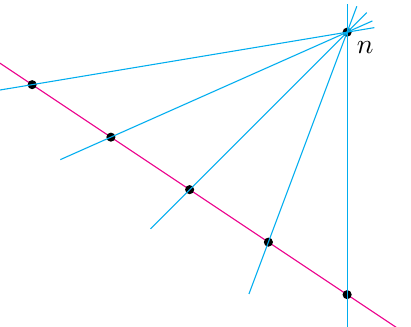
\begin{tikzpicture}
			% Draw the line
			\draw[magenta, shorten >=-100pt, shorten <=-20pt] (-2,4/3) -- (2,-4/3);
			
			% Draw a point above and to the right of the line
			\filldraw (2,2) circle (0.05) node[below right] {$n$};
			
			% Draw series of points on the line
			\foreach \x in {-2,-1,0,1,2} {
				\filldraw (\x,-\x*2/3) circle (0.05);
			}
			
			% Draw lines from each point to the point off the line
			\foreach \x in {-2,-1,0,1,2} {
				\draw[cyan, shorten >=-10pt, shorten <=-20pt] (\x,-\x*2/3) -- (2,2);
			}
		\end{tikzpicture}
		\]
		\item $\mathcal{F}$ son las líneas de un plano proyectivo finito.
	\end{itemize}
\end{teo}
\chapter{Cuadrados latinos}
\begin{defn}
	Un \textbf{cuadrado latino} de \textbf{orden} $n$ es una matrix de $n\times n$ tal que cada entrada está en un único renglón y una única columna. Dos cuadrados latinos son \textbf{ortogonales} si al sobreponerlos, ninguna de las $n^2$ entradas es igual. Una \textbf{familia ortogonal} de cuadrados latinos es una colección de cuadrados latinos mutualmente ortogonales, y se denota $\MOLS(n,k)$ donde $n$ es el orden $k$ el tamaño de la familia.
\end{defn}
\begin{lema}
	Una familia ortogonal de cuadrados latinos de orden $n$ tiene como máximo $n-1$ elementos.
\end{lema}
\begin{proof}
	Primero renombramos todos los cuadrados de la familia para que el primer renglón tenga los símbolos en orden ascendente. Esto hace que cualquier pareja de cuadrados sobrepuestos tenga las entradas $(1,1),(2,2),\ldots,(n,n)$ en el primer renglón.
	
	Ahora tomemos un cuadradito abajo del primer renglón en cualquier cuadrado latino. Cuando le ponemos encima otro cuadrado de la familia, ese cuadradito debe tener una entrada de la forma $(i,j)$ con $i\neq j$, porque todas las entradas iguales ya fueron consideradas en el primer renglón. Luego, hay uno tipo de entrada distinto para cada cuadrado en la familia, y hay $n-1$ posibles entradas.
\end{proof}
\begin{defn}
	Una familia de cuadrados latinos de orden $n$ se llama \textbf{completa} si tiene $n-1$ elementos. 
\end{defn}
\begin{teo}
	Para cualquier $n$ potencia de primo, hay una $\MOLS(n,n-1)$.
\end{teo}

\chapter{Teorema de Hall}
\begin{defn}
	Sean $A_1,\ldots,A_n$ conjuntos. Un \textbf{sistema de representantes distintos (SDR)} es una $n$-tupla $(x_1,\ldots,A_n)$ tal que:
	\begin{itemize}
		\item[(a)] $x_i\in A_i$ para toda $i$.
		\item[(b)] $x_i\neq x_j$ para toda $i\neq j$.
	\end{itemize}
\end{defn}
Es claro que para cualquier subconjunto $J$ de $\{1,\ldots,n\}$, $\left|\bigcup_{i\in J}A_i\right|\geq|J|$, pero el converso también es cierto:
\begin{teo}[de Hall]
	Existe un SDR para los conjuntos finitos $A_1,\ldots,A_n$ si y sólo si 
	\[\left|\bigcup_{i\in J}A_i\right|\geq|J|\]
	para cualquier $J\subseteq\{1,\ldots,n\}$.
\end{teo}
Dados un conjunto de niñas y uno de niños, dado que cada niño conoce cierto subconjunto de niñas, es posible casar a cada niño con una niña que conoce si y sólo si cualquier $k$-subconjunto de niños corresponde hay al menos $k$ niñas que todos ellos conocen. Es el teorema de matrimonio de Hall.
\begin{teo}
	Supongamos que los conjuntos $A_1,\ldots,A_n$ satisfacen la condición de Hall, y además $|A_i|\geq r$ para toda $i$ y algún número $r$. Entonces, la cantidad de SDRs que hay es al menos:
	\[\begin{cases}
		r!\qquad&\text{si }r\leq n\\
		r(r-1)\ldots(r-n+1)=\frac{r!}{n!}&\text{si }r>n
	\end{cases}\]
\end{teo}
\begin{teo}
	Supongamos que $A_1,\ldots,A_n$ son subconjuntos de $\{1,\ldots,n\}$ y $r$ es un entero positivo tal que
	\begin{itemize}
		\item[(a)] $|A_i|=r$ para toda $i$.
		\item[(b)] Cualquier elemento de $\{1,\ldots,n\}$ está contenido en exactamente $r$ de los subconjuntos.
	\end{itemize}
	Entonces, la familia satisface la condición de Hall, así que tiene un SDR.
\end{teo}
\begin{coro}
	Esta familia tiene $r!$ SDRs.
\end{coro}
Estos resultados se usan para completar cuadrados latinos. Ver Proofs from the Book.
\chapter{Diseños de bloques}
\begin{defn}
	Un $t$-$(v,k,\lambda)$\textbf{-diseño de bloques} es una colección $\mathcal{B}$ de subconjuntos de algún conjunto $V$ tales que:
	\begin{itemize}
		\item $V$ tiene $v$ elementos.
		\item Cada bloque en $\mathcal{B}$ tiene $k$ elementos.
		\item Cualquier familia de $t$ elementos en $V$ está en exactamente $\lambda$ bloques en común.
	\end{itemize}
\end{defn}
\begin{defn}
	La \textbf{matriz de incidencia} de un diseño de bloques es una matriz de ceros y unos cuyos renglones son los elementos de $V$ y las columnas son los bloques que indica si un elemento está en ese bloque.
\end{defn}
\begin{prop}
	Un $(v,k,\lambda)$-diseño de bloques que tiene $b$ bloques y cualquier elemento de $V$ aparece en $r$ bloques satisface que:
	\begin{enumerate}
		\item $vr=kb$
		\item $\lambda(v-1)=r(k-1)$
	\end{enumerate}
\end{prop}
\begin{proof}\leavevmode
	\begin{enumerate}
		\item Ambos lados de la igualdad son formas de contar la cantidad de 1's en la matriz de incidencia.
		\item Dado $x\in V$, ambos lados de la igualdad son formas de contar la cantidad de elementos que hay en cada bloque sin contar a $x$.
	\end{enumerate}
\end{proof}
Hay una generalización de la proposición anterior para diseños de bloques con $t\neq2$:
\begin{prop}
	Si un $t$-$(v,k,\lambda)$-diseño de bloques existe, entonces el siguiente número es un entero para $0\leq s\leq t$:
	\[\lambda\frac{{v-s\choose t-s}}{{k-s\choose t-s}}=\lambda\frac{(v-s)(v-s-1)\ldots(v-t+1)}{(k-s)(k-s-1)\ldots(k-t+1)}\]
\end{prop}
Los casos $s=0$ y $s=1$ corresponden a los incisos 1 y 2 de la primera proposición.
\begin{teo}[Desigualdad de Fisher]
	Si $k<v$, entonces $b\geq v$.
\end{teo}
\begin{proof}
	Consideramos la matriz de incidencia $A$, cuya entrada $i,j$ es
	\[a_{ij}=\begin{cases}
		1\qquad\text{si }x_i\in B_j\\
		0\qquad\text{si }x_i\notin B_j
	\end{cases}\]
	Luego, la matriz $AA^T$ tiene entrada $i,j$
	\[m_{ij}=\sum_{k=1}^ba_{ik}a_{jk}\]
	que representa la cantidad de bloques en donde están al mismo tiempo los elementos $x_i$ y $x_j$. Por definición, esta cantidad es
	\[m_{ij}=\begin{cases}
		\lambda\qquad\text{si }i\neq j\\
		r\qquad\text{si }i=j
	\end{cases}\]
	Esta matriz tiene determinante distinto de cero (usando la hipótesis $k<v$, haciendo cuentas), por lo que al ser una matriz de $v\times v$ tiene rango, es decir, la dimensión del espacio lineal generado por las columnas, igual a $v$.
	
	Para concluir notemos que \textcolor{red}{(why?)} si $b<v$, entonces el rango de $A$ y de $A^T$ sería menor estricto que $v$. Como el rango del producto es menor o igual al mínimo de los rangos de los factores, $\ran M<v$, que no es posible.
\end{proof}
Este teorema sirve para descartar la existencia de ciertos diseños de bloques, como por ejemplo $2-(16,6,1)$.

En fin,
\begin{defn}
	Un diesño de bloques es \textbf{simétrico} si $v=b$, que implica que $r=k$.
\end{defn}
Va a resultar que podremos voltear el diseño. Ahí va:
\begin{prop}
	En un diseño de bloques simétrico, no sólo cada pareja de elementos está en $\lambda$ bloques, sino que cada pareja de bloques se intersecta en $\lambda$ elementos.
\end{prop}
\begin{proof}
	Tomemos un bloque arbitrario $B$ y veamos que su intersección con todos los demás es de tamaño $\lambda$. Denotemos por $x_i,\ldots,x_{v-1}$ el tamaño de la intersección de $B$ con el $i$-ésimo bloque. Mostraremos que $\sum(x_i-\lambda)^2=0$.
	
	Cada elemento de $B$ está en $k-1$ bloques además de $B$. Así que hay $k(k-1)$ elementos en la intersección de $B$ con algún otro bloque, es decir, $\sum x_i=k(k-1)=\lambda(v-1)$ aplicando nuestra proposición.
	
	Análogamente, cada pareja en $B$ está en $\lambda -1$ bloques además de $B$, así que hay ${k\choose 2}(\lambda-1)$ parejas en la intersección de $B$ con otro bloque, es decir, $\sum{x_i\choose 2}={k\choose 2}(\lambda-1)$. Podemos reescribir esto como $\sum x_i(x_i-1)=k(k-1)(\lambda-1)=\sum x_i^2-x_i=\lambda(v-1)(\lambda-1)$.
	
	Sumando las dos igualdades obtenemos que $\sum x_i^2=\lambda(v-1)+\lambda(v-1)(\lambda-1)=\lambda^2(v-1)$. Y luego:
	\begin{align*}
		\sum(x_i-\lambda)^2&=\sum x_i^2-2\sum\lambda x_i+\sum \lambda^2\\
		&=\lambda^2(v-1)-2\lambda(\lambda(v-1))+(v-1)\lambda^2=0
	\end{align*}
\end{proof}
\begin{prop}
	En un diseño de bloques simétrico, si $v$ es par, entonces $k-\lambda$ es un cuadrado.
\end{prop}
\begin{teo}[Bruck-Ryser-Chowla]
	Si existe un $(v,k,\lambda)$-diseño de bloques simétrico, entonces
	\begin{enumerate}
		\item[\textit{(a)}] Si $v$ es par, $k-\lambda$ es un cuadrado.
		\item[\textit{(b)}] Si $v$ es impar, entonces
		\[z^2=(k-\lambda)x^2+(-1)^{(v-1)/2}\lambda y^2\]
		tiene una solución entera no cero en $x,y,z$.
	\end{enumerate}
\end{teo}
\chapter{Matrices de Hadamard}
¿Qué tan grande puede ser el determinante de una martiz cuyas entradas están acotdadas?
\begin{teo}[de Hadamard]
	Sea $A$ una matriz de $n\times n$ de números reales tal que $|a_{ij}|\leq1$ para toda $i,j$. Entonces, $\det A\leq n^{n/2}$, y la igualdad se satisface si y sólo si $a_{ij}=\pm1$ y $AA^T=nId$.
\end{teo}
\begin{proof}
	El determinante es el volumen del paralelepípedo $n$-dimensional cuyos lados son los renglones de $A$. Este volumen es menor o igual al producto del tamaño de los lados, que es $\sqrt{\sum_{j=1}^n a_{ij}^2}$ para el $i$-ésimo renglón. Este número es menor o igual que $\sqrt{n}$, así que se sigue la desigualdad. La igualdad se tiene sólo cuando los lados son justo de ese tamaño, por lo que $|a_{ij}|=1$, y además los lados del paralelepípedo son perpendiculares entre sí, de forma que $\sum_{k=1}^na_{ik}a_{jk}=0$. Esto es tanto como decir que $AA^T=nId$.
\end{proof}
\begin{defn}
	Una matriz que satisface la igualdad en el teorema anterior es una \textbf{matriz de Hadamard}.
\end{defn}
\begin{prop}
	Si existe una matriz de Hadamard de orden $n$, entonces $n=1$ o $2$, o bien $n\equiv0\mod4$.
\end{prop}
\begin{teo}
	Si $n>4$, son equivalentes:
	\begin{itemize}
		\item Existe una matriz de Hadamard de orden $n$.
		\item Existe un $3$-$(n,\frac{1}{2}n,\frac{1}{2}n-1)$-diseño de bloques.
		\item Existe un $2$-$(n-1,\frac{1}{2}n-1,\frac{1}{4}n-1)$-diseño de bloques.
	\end{itemize}
\end{teo}
\chapter{Planos proyectivos finitos}
\begin{defn}
	Un \textbf{plano proyectivo finito} es una pareja $(\mathcal{P},\mathcal{L})$ donde $\mathcal{P}$ es un conjunto finito de \textit{puntos} y $\mathcal{L}$ es una familia de \textit{líneas}, subconjuntos de $\mathcal{P}$, tales que
	\begin{itemize}
		\item[\textbf{(P0)}] Hay cuatro puntos en posición general.
		\item[\textbf{(P1)}] Cualesquiera dos líneas se intersectan en un único punto.
		\item[\textbf{(P2)}] Por cualesquiera dos puntos pasa una única línea.
	\end{itemize}
\end{defn}
\begin{lema}
	Dadas dos líneas, hay un punto que no está en ellas.
\end{lema}
\begin{proof}
	Cada una de nuestras dos líneas puede intersectar al conjunto de cuatro puntos no colineales, llamémoslo $F$, en a lo más dos puntos. Si uno de estos cuatro puntos está fuera de las dos líneas, terminamos, y si no, nuestras dos líneas están generadas por dos parejas en $F$, digamos $\ell =F^1_\ell\vee F^2_\ell$ y $m=F^1_m\vee F^2_m$. Ahora tomemos las parejas $F^1_\ell\vee F^1_m:=a$ y $F^2_\ell\vee F^2_m:=b$. Si el punto $P=a\wedge b$ está en $\ell$, entonces $F^1_\ell$, $F^2_\ell$ y $F^1_m$ estarían en la misma línea, pero esto no es posible. Lo mismo sucede para $m$.
\end{proof}
\[ 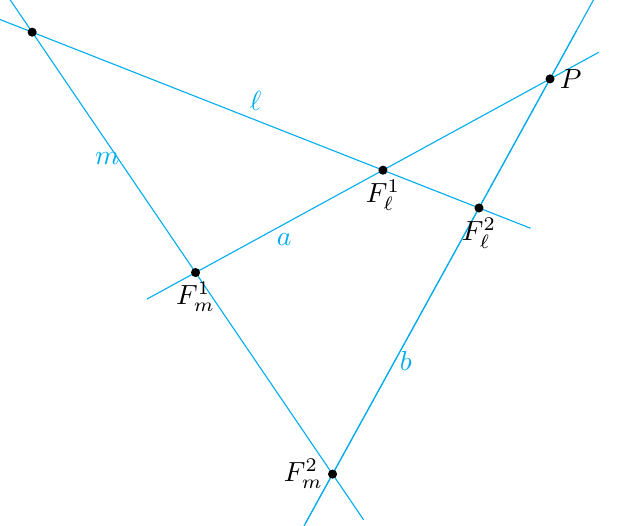
\begin{tikzpicture}
	% Lines
	\draw[cyan, shorten >=-20pt, shorten <=-20pt] (-2.04,-1.42) -- (2.4619664439073, 1.0390573012939) node[near start, below] {$a$};
	\draw[cyan, shorten >=-100pt, shorten <=-70pt] (-0.3,-3.98) -- (1.56,-0.6) node[midway, below] {$b$};
	\draw[cyan, shorten >=-20pt, shorten <=-20pt] (1.56,-0.6) -- (-4.1149195804196, 1.6327552447552) node[midway, above] {$\ell$};
	\draw[cyan, shorten >=-50pt, shorten <=-20pt] (-0.3,-3.98) -- (-4.1149195804196, 1.6327552447552) node[near end, below] {$m$};
	\draw[cyan, shorten >=-20pt, shorten <=-20pt] (-0.3,-3.98) -- (2.4619664439073, 1.0390573012939);
	% Points
	\filldraw (-0.3,-3.98) circle (0.05) node[left] {$F^2_m$};
	\filldraw (1.56,-0.6) circle (0.05) node[below] {$F^2_\ell$};
	\filldraw (0.34,-0.12) circle (0.05) node[below] {$F^1_\ell$};
	\filldraw (-2.04,-1.42) circle (0.05) node[below] {$F^1_m$};
	\filldraw (-4.1149195804196, 1.6327552447552) circle (0.05);
	\filldraw (2.4619664439073, 1.0390573012939) circle (0.05) node[right] {$P$};
\end{tikzpicture}\]

%\[\begin{tikzpicture}
%	% Points
%	\filldraw (-0.3,-3.98) circle (0.05) node[below] {$A$};
%	\filldraw (1.56,-0.6) circle (0.05) node[right] {$B$};
%	\filldraw (0.34,-0.12) circle (0.05) node[right] {$C$};
%	\filldraw (-2.04,-1.42) circle (0.05) node[left] {$D$};
%	\filldraw (-4.1149195804196, 1.6327552447552) circle (0.05) node[left] {$E$};
%	\filldraw (2.4619664439073, 1.0390573012939) circle (0.05) node[right] {$F$};
%	
%	% Lines
%	\draw[cyan] (-2.04,-1.42) -- (2.4619664439073, 1.0390573012939) node[midway, above] {$f$};
%	\draw[cyan] (-0.3,-3.98) -- (1.56,-0.6) node[midway, above] {$g$};
%	\draw[cyan] (1.56,-0.6) -- (-4.1149195804196, 1.6327552447552) node[midway, above] {$h$};
%	\draw[cyan] (-0.3,-3.98) -- (-4.1149195804196, 1.6327552447552) node[midway, above] {$i$};
%	\draw[cyan] (-0.3,-3.98) -- (2.4619664439073, 1.0390573012939) node[midway, above] {$j$};
%	\draw[cyan] (-0.3,-3.98) -- (0.34,-0.12) node[midway, above] {$k$};
%	\draw[cyan] (-2.04,-1.42) -- (1.56,-0.6) node[midway, above] {$l$};
%\end{tikzpicture}\]
\begin{prop}
	Todas las líneas tienen la misma cantidad de puntos.
\end{prop}
\begin{proof}
	Tomemos dos líneas $\ell,m\in\mathcal{L}$ y un punto $Z$ que no está en ninguna de ellas. Definamos la proyección que envía un punto $X\in\ell$ en el punto de intersección de la recta $XZ$ con $m$.
	\[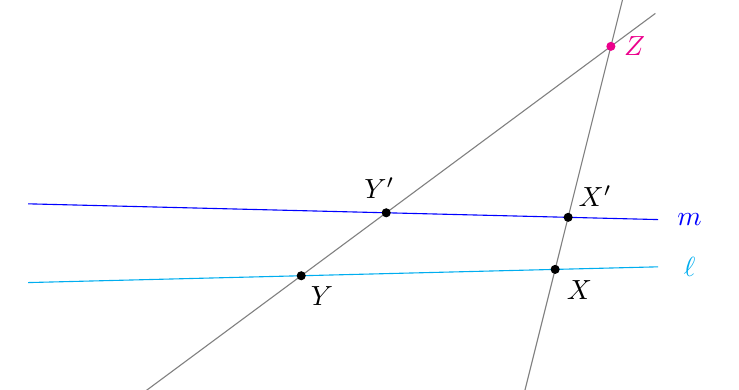
\begin{tikzpicture}
		\draw[blue] (-5,0)--(3,-0.2) node at (3.4,-0.2) {$m$};
		\draw[cyan] (-5,-1)--(3,-0.8) node at (3.4,-0.8) {$\ell$};
		
		\draw[gray,shorten >=-50pt, shorten <=-20pt] (2.4,2)--(-3,-2);
		\draw[gray,shorten >=-40pt, shorten <=-100pt] (2.4,2)--(1.4,-2);
		
		\filldraw[magenta] (2.4,2) circle (0.05) node at (2.7,2){$Z$};
		\filldraw (-0.453446191052, -0.1136638452237) circle (0.05)node at (-0.54,0.2) {$Y'$};
		\filldraw (1.6918238993711, -0.8327044025157)circle (0.05)node at (2,-1.1) {$X$};;
		\filldraw (-1.5329883570505,-0.9133247089263)circle (0.05) node at (-1.27,-1.17) {$Y$};
		\filldraw (1.8571428571429, -0.1714285714286)circle (0.05)node at (2.2,0.1) {$X'$};
	\end{tikzpicture}\]
	Por (P1), la recta $XZ$ intersecta a $m$ en un sólo punto, así que la función está bien definida. Además, es inyectiva, pues si dos de estas líneas se intersectan en el mismo punto de $m$, entonces los dos puntos en $\ell$ de los que provienen, digamos $X$ y $Y$, de no ser iguales, obligarían a $Z$ a estar en $\ell$: sólo una línea pasa por ellos (P2).
\end{proof}
\begin{prop}
	La cantidad de puntos que hay en cada línea es igual para todos los puntos, y de hecho es igual a la cantidad de líneas que pasan por cada punto.
\end{prop}
\begin{proof}
	Un momento por favor.
\end{proof}
\begin{defn}
	El \textbf{orden} del plano proyectivo es el tamaño de las líneas menos 1.
\end{defn}
\begin{prop}
	Una familia de conjuntos de tamaño $q+1$ es la colección de líneas de un plano proyectivo de orden $q$ si y sólo si es un $(q^2+q+1,q+1,1)$-diseño de bloques.
\end{prop}
\begin{proof}\leavevmode
	
	($\implies$) Las condiciones \textbf{2} y \textbf{3} de la definición se satisfacen trivialmente. Para ver la primera, tomemos una línea $\ell\in\mathcal{L}$. Para cada uno de los $q+1$ puntos en ella pasa una línea distinta de $\ell$. Esto hace que haya exactamente $1+(q+1)q=q^2+q+1$ líneas.
	
	($\impliedby$) La condición que cualesquiera dos elementos en $V$ se intersecten en un sólo bloque nos da la propiedad \textbf{(P2)}. Usando las fórmulas $vr=kb$ y $\lambda(v-1))=r(k-1)$, obtenemos que $v=b$ y $r=k$. Es decir, la cantidad de bloques es igual a la cantidad de puntos, y cada punto está en tantos bloques como puntos en cada bloque hay. Estas dos frases implican que el diseño de bloques es simétrico, luego, se sigue que cada pareja de bloques se intersecta en $\lambda=1$ puntos.
\end{proof}
\begin{prop}
	El \textbf{dual} de un plano proyectivo, la esctructura que obtenemos al intercambiar los papeles de la líneas y los puntos preservando incidencia, también es un plano proyectivo.
\end{prop}
\chapter{Ternas de Steiner}
Los planos proyectivos son los diesños de bloques con $k$ más grande. Las ternas de Steiner tienen el $k$ más pequeño: tres.
\begin{prop}[Cameron, 8.1.1]Sea $\mathcal{B}$ una familia de $m$-subconjuntos de un $n$-conjunto tal que cualquier $l$-subconjunto está contenida en a lo más un elemento de $\mathcal{B}$. Entonces
	\[|\mathcal{B}|\leq{n\choose l}\Big/{m\choose l}\]
	y la igualdad se da cuando cada $l$-subconjunto está contenido en exactamente un elemento de $\mathcal{B}$.
\end{prop}
\begin{proof}
	Para la igualdad, se trata de un $l$-$(n,m,1)$-diseño de bloques. Cualquier subconjunto de tamaño $l$ está contenido en exactamente un $m$-bloque. En este caso, los $l$-subconjuntos del $n$-conjunto están en correspondencia con los $l$-subconjuntos de los bloques. Cada bloque tiene ${m\choose l}$ $l$-subconjuntos.
	
	Si cada $l$ subconjunto está en a lo más un elemento de $|B|$, puede haber más $l$-subconjuntos en total que los que les hacemos corresponder en los bloques.
\end{proof}
\begin{defn}
	Una \textbf{terna de Steiner} es un $(v,3,1)$-diseño de bloques, denotado por $\STS(v)$.
\end{defn}
\begin{teo}
	Si un $\STS(v)$ existe, entonces $v=1,3\mod6$
\end{teo}
\begin{proof}
	Sustituyendo los valores conocidos en nuestras fórmulas, obtenemos que
	\[\lambda(v-1)=r(k-1)\approx\frac{v-1}{2}=r\qquad\implies\qquad vr=kb\approx \frac{v(v-1)}{6}=b\]
	La primera igualdad quiere decir que $v$ es impar, así que debe estar en alguna de las clases equivalencia $\bar{1},\bar{3}$ o $\bar{5}$ en $\Z_6$. Para ver que no puede ser $\bar{5}$, supongamos que $v=6m+5$. Entonces tenemos:
	\[\frac{(6m+5)(6m+4)}{6}=\frac{(6m+5)(3m+2)}{3}\]
	pero ni $6m+5$ ni $3m+2$ son múltiplos de $3$, así que esa fracción no podría ser un entero, que no es posible.
\end{proof}

\chapter{Ejercicios}

\end{document}